\subsection{Fixed point C models}
\label{subs:C model}

After the development of the IIR filter in Matlab environment, a C language version was implemented to evaluate the performance of the filter in arithmetic \textit{Fixed-point}. For this purpose it was used the C language program available on the teaching portal called \textit{myfilterii.c}, to which were passed from the command line the sample file generated by Matlab and the file to save the output samples from the filter implemented in C language. The program produced an output file that was then analyzed in Matlab environment to evaluate the Total Harmonic Distortion(THD). Having chosen an initial representation of the 10 bits coefficients, the following THDs presented in \autoref{fig:THD_10_bit_FL_P} have been obtained respectively with the output signal obtained on Matlab and then obtained in C fixed point arithmetic:

\begin{figure}[ht]
	\begin{minipage}[b]{0.5\linewidth}
		\centering
		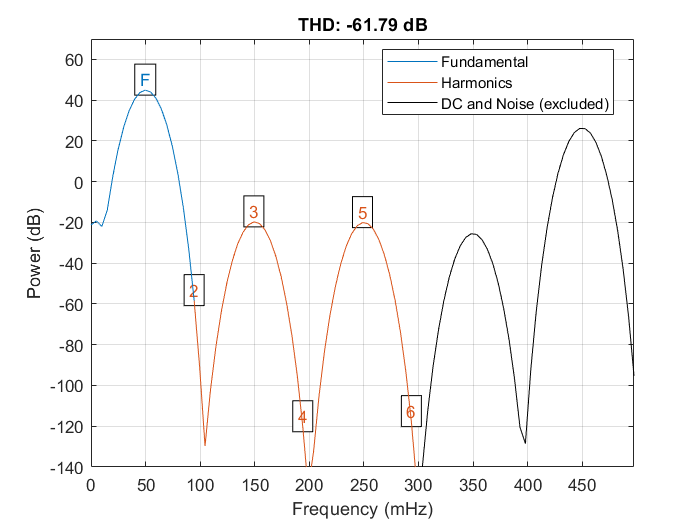
\includegraphics[width=\textwidth]{THD_10_bit_matlab_result.png}
		\caption{THD with Floating point arithmetic}
		\label{fig:THD_10_bit_FL_P}
	\end{minipage}
	\hspace{0.5cm}		
	\begin{minipage}[b]{0.5\linewidth}
		\centering
		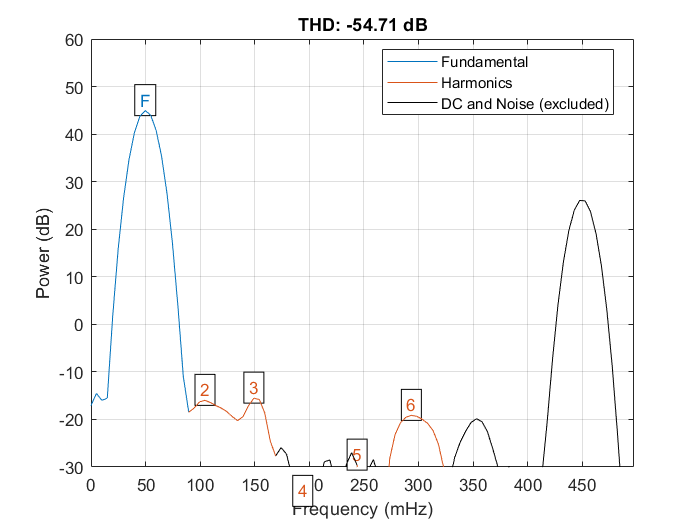
\includegraphics[width=\textwidth]{THD_10_bit_C_result.png}
		\caption{THD with 10 bit Fixed Point arithmetic}
		\label{fig:THD_10_bit_FIX_P}
	\end{minipage}
\end{figure}

As can be seen from the graph in \autoref{fig:THD_10_bit_FIX_P}, the Total Harmonic Distortion of the filter that made use of coefficients and signal represented on 10 bits is too high compared to the assigned specifications. Therefore the process described above has been iterated, using at each cycle one bit less in the representation, until the optimal value of bits has been obtained that allows to remain within the specifications of the \textit{THD}, which corresponds to 5 bits.
Then the THDs graphs have been reported, respectively calculated with the output signal obtained on Matlab and followed by the one evaluated with the fixed point arithmetic in C:

\begin{figure}[ht]
	\begin{minipage}[b]{0.5\linewidth}
		\centering
		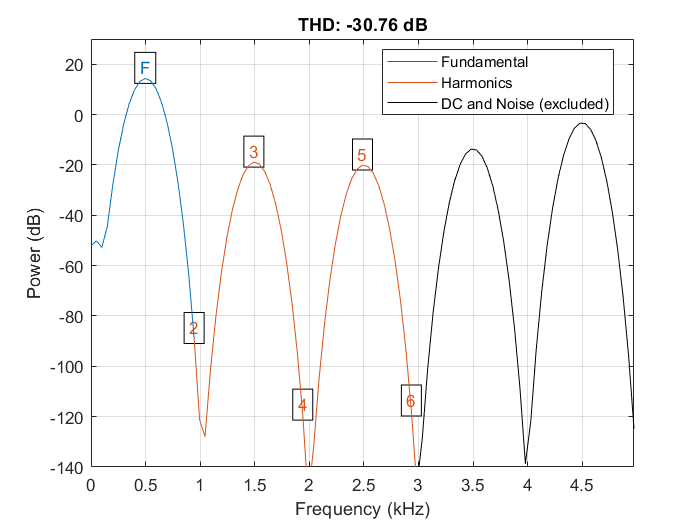
\includegraphics[width=\textwidth]{THD_5_bit_matlab_result.png}
		\caption{THD with Floating point arithmetic}
		\label{fig:THD_5_bit_FL_P}
	\end{minipage}
	\hspace{0.5cm}
	\begin{minipage}[b]{0.5\linewidth}
		\centering
		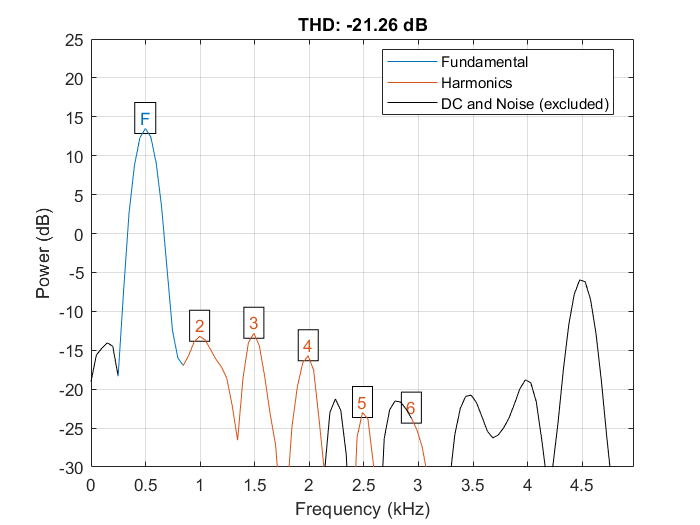
\includegraphics[width=\textwidth]{THD_5_bit_C_result.png}
		\caption{THD with 5 bit Fixed Point arithmetic}
		\label{fig:THD_5_bit_FIX_P}
	\end{minipage}
\end{figure}

\noindent The final value of THD is therefore $-21.26 dB$ which is perfectly in line with the assigned project specifications.
From the graphs in \autoref{fig:Allan_Var_DF2}, it can be seen that in the first half of the observation window the signal has a high noise, generating a low stability of the oscillator, but over time it seems to weaken, increasing its frequency stability. From the difference of the two graphs instead we can notice that the frequency behavior of the two signals is very similar, because the difference of their variances is much below the order of magnitude of the unit.